% !TeX program = xelatex
% Compile in this directory: latexmk -xelatex pyfracpaq-user-manual-en.tex
\documentclass[11pt,a4paper,oneside,parskip=half]{scrartcl}
\newcommand{\ManualTitle}{User manual}
\newcommand{\ManualDate}{November 2026}
\newcommand{\ManualAuthor}{PyFracPaQ documentation}
\newcommand{\ManualSubject}{Usage, methods and SD11A worked examples}
\usepackage[british]{babel}
% Shared layout and typography for both language editions.
\usepackage[margin=23mm,headheight=16pt,footskip=12mm]{geometry}
\usepackage{fontspec}
\setmainfont{texgyrepagella}[Extension=.otf,UprightFont=*-regular,BoldFont=*-bold,ItalicFont=*-italic,BoldItalicFont=*-bolditalic]
\setsansfont{texgyreheros}[Extension=.otf,UprightFont=*-regular,BoldFont=*-bold,ItalicFont=*-italic,BoldItalicFont=*-bolditalic]
\setmonofont[Scale=.86]{lmmono10-regular.otf}
\usepackage{unicode-math}
\setmathfont{texgyrepagella-math.otf}
\usepackage{graphicx,booktabs,tabularx,longtable,array}
\usepackage[dvipsnames]{xcolor}
\usepackage{enumitem,microtype,needspace,placeins,fancyhdr,lastpage,xurl}
\usepackage[most]{tcolorbox}
\definecolor{brand}{HTML}{126870}
\definecolor{ink}{HTML}{18323A}
\definecolor{pale}{HTML}{F0F6F6}
\usepackage[colorlinks=true,linkcolor=brand,urlcolor=brand,citecolor=brand,bookmarksnumbered=true,pdfencoding=auto]{hyperref}
\hypersetup{pdftitle={PyFracPaQ 0.9.0rc1 - \ManualTitle},pdfauthor={\ManualAuthor},pdfsubject={\ManualSubject}}
\graphicspath{{assets/}}
\setlength{\emergencystretch}{3em}
\setcounter{tocdepth}{2}
\setlist{nosep,topsep=5pt,leftmargin=*}
\setkomafont{section}{\sffamily\bfseries\color{brand}\Large}
\setkomafont{subsection}{\sffamily\bfseries\color{ink}\large}
\setkomafont{subsubsection}{\sffamily\bfseries\normalsize}
\pagestyle{fancy}\fancyhf{}
\fancyhead[L]{\small\sffamily PyFracPaQ / \ManualTitle}
\fancyhead[R]{\small\sffamily 0.9.0rc1}
\fancyfoot[L]{\footnotesize \ManualDate}
\fancyfoot[R]{\footnotesize\thepage\ / \pageref*{LastPage}}
\renewcommand{\headrulewidth}{.3pt}
\fancypagestyle{plain}{\fancyhf{}\fancyhead[L]{\small\sffamily PyFracPaQ / \ManualTitle}\fancyhead[R]{\small\sffamily 0.9.0rc1}\fancyfoot[L]{\footnotesize \ManualDate}\fancyfoot[R]{\footnotesize\thepage\ / \pageref*{LastPage}}\renewcommand{\headrulewidth}{.3pt}}
\raggedbottom
\renewcommand{\arraystretch}{1.12}
\newcommand{\control}[1]{\textsf{#1}}
\newcommand{\code}[1]{{\small\texttt{\detokenize{#1}}}}
\newcommand{\major}[1]{\FloatBarrier\clearpage\section{#1}}
\newcommand{\feature}[2]{\FloatBarrier\Needspace{5\baselineskip}\subsection{#2}\label{feat:#1}}
\newcommand{\plotfig}[3]{\begin{figure}[htbp]\centering\includegraphics[width=.82\linewidth]{#1}\caption{#2}\label{#3}\end{figure}}
\newcommand{\uifig}[3]{\begin{figure}[htbp]\centering\includegraphics[width=.72\linewidth]{#1}\caption{#2}\label{#3}\end{figure}}
\newtcolorbox{note}[1]{colback=pale,colframe=brand,boxrule=.5pt,arc=1mm,title={#1},fonttitle=\sffamily\bfseries}

\begin{document}
\begin{titlepage}
\thispagestyle{empty}
\vspace*{13mm}

\includegraphics[width=.54\linewidth]{logo.png}\par
\vspace{18mm}
{\Huge\sffamily\bfseries\color{ink} User manual\par}
\vspace{5mm}
{\Large Usage, methods and SD11A worked examples\par}
\vspace{10mm}
{\large PyFracPaQ 0.9.0rc1\par}
{\large November 2026\par}
\vspace{12mm}
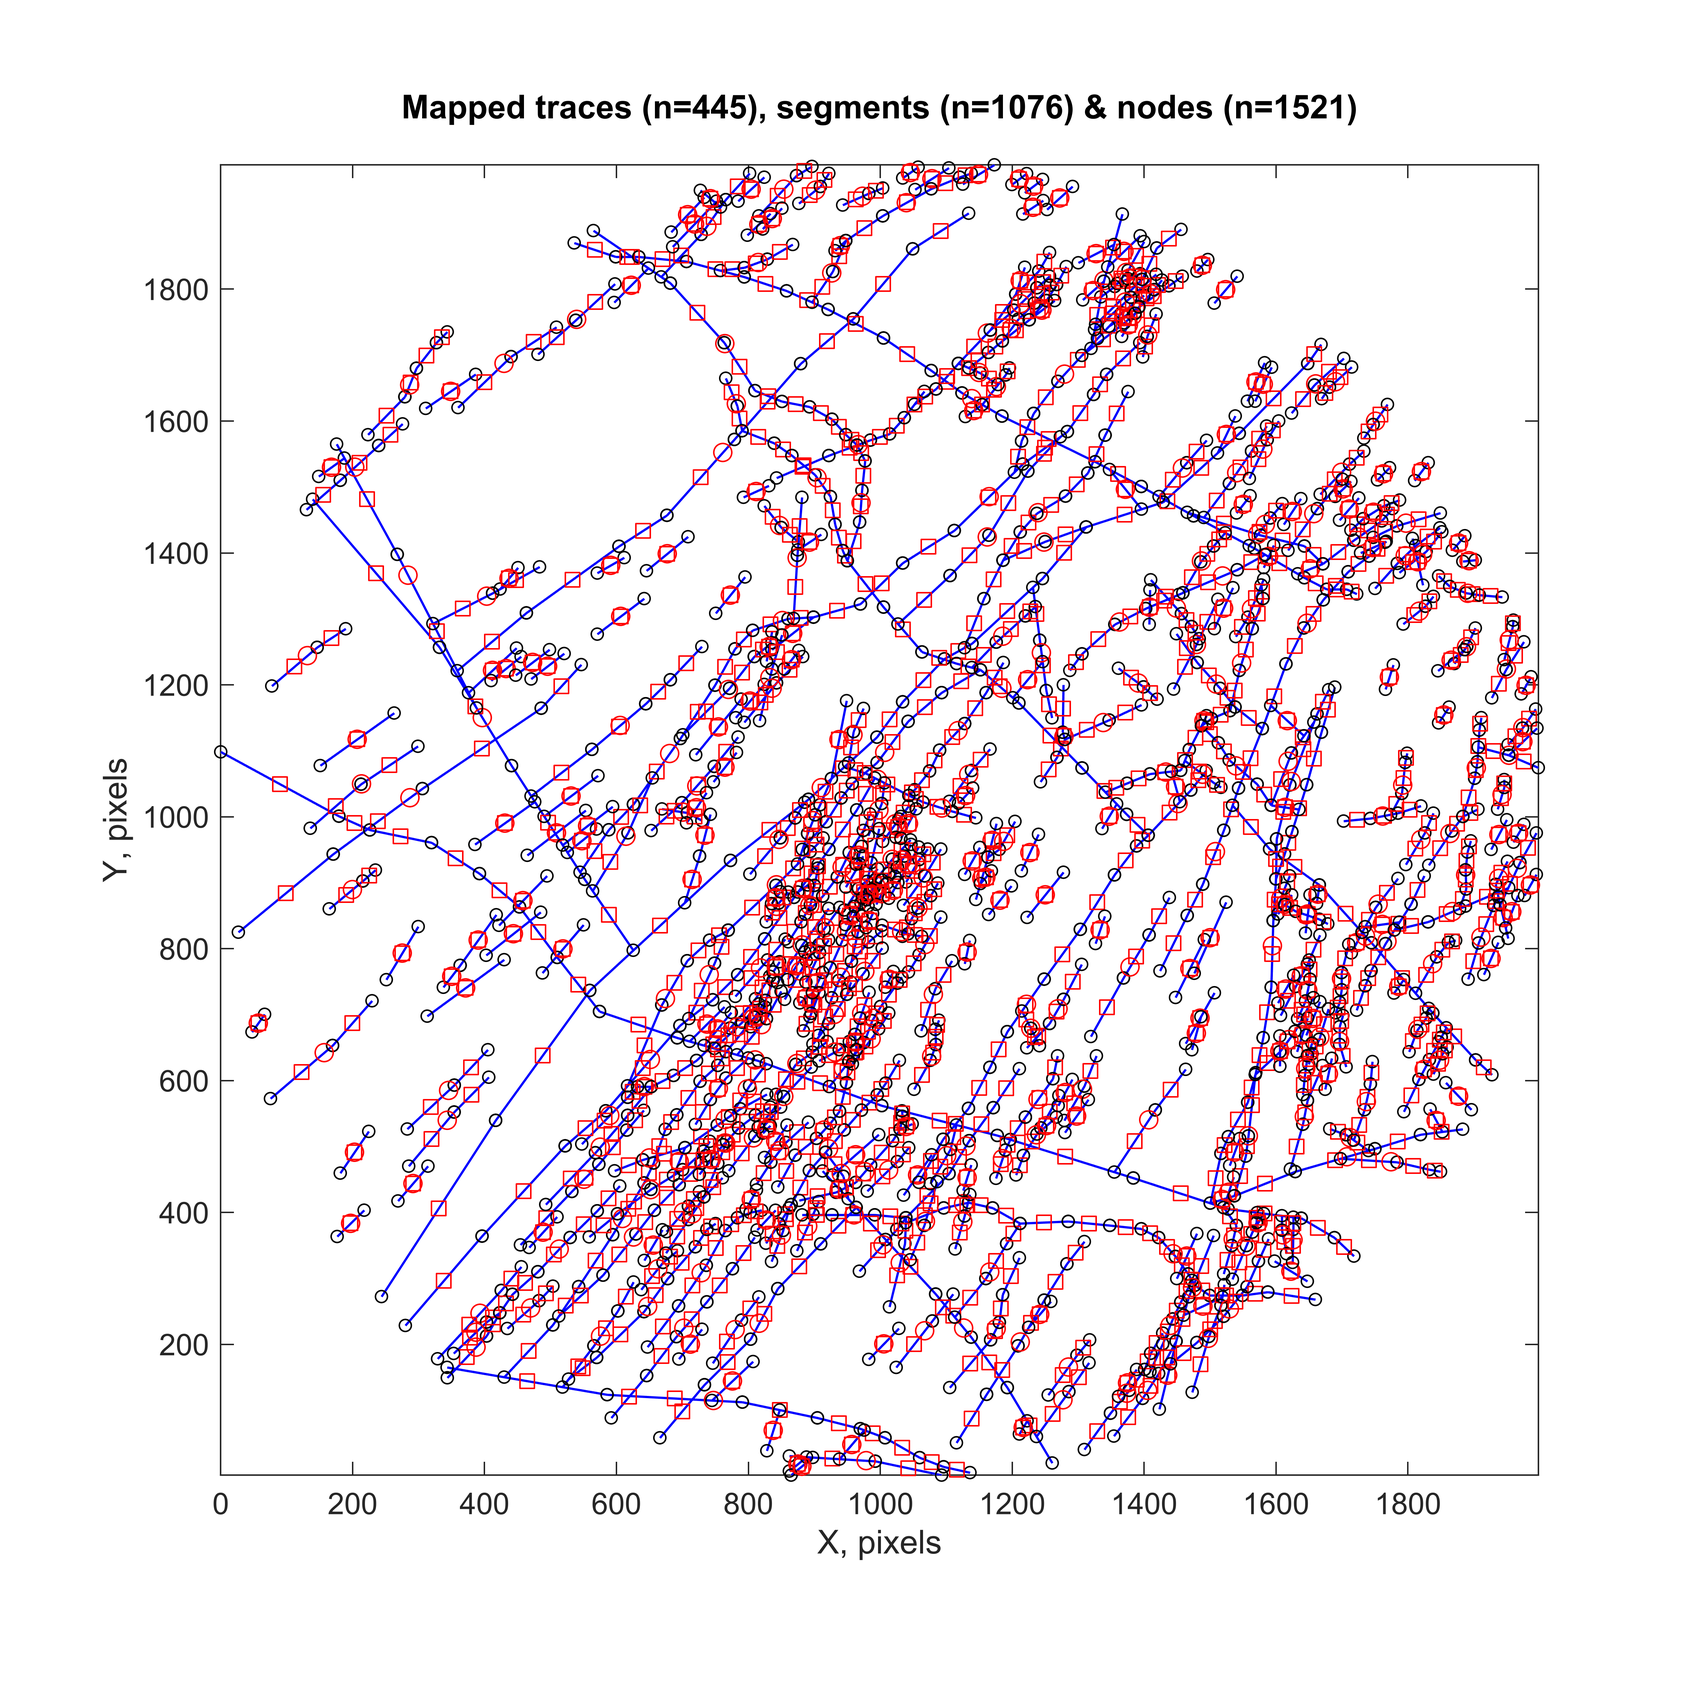
\includegraphics[width=.60\linewidth]{tracemap.png}
\vfill
{\small Python implementation based on FracPaQ MATLAB 2.8.\par
Run the code locally; MATLAB is not required.\par
Contact: \href{mailto:luismauricio@me.com}{luismauricio@me.com}.}
\end{titlepage}
\section*{How to use this manual}
\addcontentsline{toc}{section}{How to use this manual}
Start with Sections~\ref{sec:inicio}--\ref{sec:roteiro} to prepare the environment, understand the inputs and run the first example. Then turn to the relevant application tab. Each feature describes its controls, calculation, interpretation and outputs. Control labels retain the wording used in the interface, including \control{Colour by strike?}.

The main example is \code{examples/SD11A.txt}, copied unchanged from the FracPaQ distribution supplied by the maintainer. The illustrated results use pixels without physical calibration. Do not interpret those pixels as metres, or the illustrative stress and aperture parameters as measurements of this sample.

The analytical figures are reviewed Python outputs. Interface captures show the actual widgets in an illustrative 1250\,\(\times\)\,739-pixel window. The application opens at the available screen width; its appearance and size can vary with the monitor. Tab panels are cropped only to improve legibility on the printed page.

\begin{note}{Scientific scope}
The application describes two-dimensional traces. Intensity, connectivity, tensors and permeability are estimates under the stated assumptions, not complete flow simulations or reconstructions of three-dimensional fractures. Section~\ref{sec:limites} summarises the approved corrections to legacy behaviour. The MATLAB reference is version 2.8; 0.9.0rc1 identifies this Python port.
\end{note}
\clearpage
\tableofcontents
% !TeX root = ../pyfracpaq-user-manual-en.tex
\major{Prepare the environment and start the application}\label{sec:inicio}
Obtain the code folder from GitHub by cloning the repository or downloading its ZIP. Open the folder containing \code{run_gui.py} and \code{requirements.txt}. Normal use requires Python 3.13 and the libraries; installing the PyFracPaQ package itself is unnecessary.

\subsection{Python and a virtual environment}
On macOS, with Python 3.13 available, run these commands from the project root:
\begin{verbatim}
python3.13 -m venv .venv
.venv/bin/python -m pip install -r requirements.txt
.venv/bin/python -m pip check
.venv/bin/python run_gui.py
\end{verbatim}
Alternatively, use \code{.venv/bin/python -m pyfracpaq} from the same folder. Obtaining the libraries may initially require internet access; subsequent analyses run locally. Do not silently change the versions pinned in requirements.txt.

\subsection{Miniforge and VS Code}
With Miniforge, prepare a separate environment:
\begin{verbatim}
conda create -n pyfracpaq python=3.13 pip
conda activate pyfracpaq
python -m pip install -r requirements.txt
python -m pip check
python run_gui.py
\end{verbatim}
In VS Code, open the folder and use \control{Python: Select Interpreter}. Select the Python executable in \code{.venv} or your Miniforge environment. Run \code{run_gui.py} or one of the supplied Run and Debug configurations. The Python extension supports selection and execution; Python Debugger is required for the debugging configurations.

CPython 3.13.18 and Miniforge/Python 3.13.13 have been checked on macOS arm64. Windows/Linux remain subject to future testing by the maintainer, rather than certified platforms. An environment already named pyfracpaq may use another version: check \code{python --version} before installing the libraries.

\subsection{What the folder needs to contain}
The application uses \code{pyfracpaq/}, its resources, the launcher and the libraries. \code{examples/} and this manual support normal use. Tests, audit reports and internal scripts are development material in the full clone and are not required at run time. The usage ZIP excludes them. The MATLAB distribution is not required.

\subsection{Working directory and existing files}
The usual output destination is the current working directory. Starting from the project root writes results there. To keep analyses separate, use a working copy or start the absolute path to \code{run_gui.py} from the output folder, using the prepared Python executable. Without installing the project, module execution should start at the project root.

Reusing a tag reuses and replaces the same filenames. Some intermediate files have fixed names without a tag. Preserve original inputs and separate analyses before clicking Run. SVG conversion is an exception to the output location: its TXT files are written beside the SVG.

\major{Inputs, geometry, scaling and orientation}\label{sec:dados}
\subsection{Traces, segments and nodes}
A \emph{trace} is the polyline representing a mapped fracture. Its vertices are input nodes; consecutive nodes define a segment. These geometric nodes are not automatically the topological I/Y/X nodes calculated later.

For \(\mathbf p_i=(x_i,y_i)\),
\begin{equation}
\ell_i=\|\mathbf p_{i+1}-\mathbf p_i\|_2,
\qquad L=\sum_i\ell_i.
\end{equation}
Total length \(L\) follows the path, rather than the straight distance between the endpoints. A trace centre is interpolated halfway along that path. A segment centre is the mean of its endpoints. These positions are used in profiles and the variogram.

The usual sampling area is the rectangular domain,
\begin{equation}
A=(x_{\max}-x_{\min})(y_{\max}-y_{\min}).
\end{equation}
Do not confuse this area with the sum of block areas. For image inputs, some analyses use the complete image domain, whereas tensors use the envelope of the extracted nodes. Each family identifies the relevant area below.

\subsection{Node TXT files}
Each line contains one trace, with X/Y pairs separated by TAB and no header. A two-trace example is:
\begin{verbatim}
0<TAB>0<TAB>4<TAB>0
1<TAB>2<TAB>4<TAB>2<TAB>4<TAB>6
\end{verbatim}
Replace \code{<TAB>} with an actual tab character. The first trace contains one segment and the second contains two. Each line requires at least two distinct nodes. Empty or non-finite values and incomplete pairs are rejected with an error location, without partial import. Consecutive duplicate nodes are removed with a diagnostic; a trace that becomes degenerate is rejected.

\subsection{Physical scaling}
Enter a known calibration \(s>0\) in \control{Scaling (pixels/metre)}. Leaving the field blank retains pixels. Geometry is rebuilt from the source:
\begin{equation}
 x_m=x_{px}/s,\quad y_m=y_{px}/s,\quad
 L_m=L_{px}/s,\quad A_m=A_{px}/s^2.
\end{equation}
This is more than changing a label. A new scale requires a new preview and clears the Graphs line. Intensity has inverse-length units, density inverse-area units and permeability area units. An aperture entered in Fluid flow must use the current length unit; changing the scale does not automatically convert the number in that field.

\subsection{Flips, north and angles}
A segment's raw angle is measured relative to the Y-axis as an axial direction, usually represented in \([0,180]\). An equivalent geometric expression is \(\beta=\operatorname{atan2}(\Delta x,\Delta y)\), with the application's axial representation. North, rounding and flips are applied by the relevant routines; they do not modify stored nodes.

\control{Flip X-axis} and \control{Flip Y-axis} reflect the display and affect angular corrections in the relevant families. \control{Rotate Y-axis from N (°)}, where used, corrects the angular reference. Graphs angle profiles and the raw angle/length TXT do not receive the same transformation as EZROSE. Wavelets operates on its raster without the north correction.

\begin{note}{Avoid correcting the geometry twice}
Do not redraw input nodes to compensate for a flip that will also be applied in the interface. Check a fracture of known orientation before interpreting roses, tensors or stresses. Differences between angular files are intentional and do not by themselves indicate a unit error.
\end{note}

\subsection{SVG: sets grouped by colour}
Supported geometry includes \code{line}, \code{polyline} and absolute M/L paths, with hexadecimal stroke colours specified as attributes, inline styles or groups. \code{examples/colours.svg} contains two colours. Curves, transformations, SVG polygons and external CSS/classes are not silently converted: prepare the file in the source editor.

Preview converts nodes to TXT files beside the SVG, grouped by colour. Filenames include \code{_colourHHHHHH_converted.txt}; a simple set uses \code{_converted.txt}. Reloading a colour-specific TXT allows individual analysis. Where applicable, a multicolour SVG adds a multicolour trace figure. Colour identifies the input set, rather than an inferred statistical class.
\plotfig{tracemap_multicolour.png}{An auxiliary SVG example, separate from SD11A: preserving colour groups in a trace map.}{fig:svg}

\subsection{Images: the Hough transform}\label{sec:hough}
Use a single-frame, eight-bit grayscale JPEG/TIFF. RGB, alpha, indexed and higher-depth images are not automatically converted by the GUI. Use the preprocessing utility when needed, and inspect its output.

The complemented image identifies non-white pixels, removes isolated pixels and applies the standard Hough transform:
\begin{equation}
\rho=x\cos\theta+y\sin\theta.
\end{equation}
A pixel line accumulates votes in \((\theta,\rho)\) space. The angular step is \(0.5^\circ\), the \(\rho\) step is one pixel and final image coordinates are one-based. This detects straight segments; it does not replace interpretative digitisation of curved fractures.

\begin{tabularx}{\linewidth}{@{}p{.35\linewidth}X@{}}
\toprule Control & Effect on image Preview\\\midrule
\control{Number of Hough peaks} & Peak limit: integer from 100 to 5000. More peaks may include noise.\\
\control{Hough threshold} & Fraction of the accumulator maximum, \(0<t\leq1\). A lower threshold retains weaker peaks.\\
\control{Merge gaps less than} & FillGap: pixel distance for joining compatible portions; greater than 1.\\
\control{Discard lengths less than} & MinLength: minimum pixel length; greater than 1.\\\bottomrule
\end{tabularx}
Defaults are 1000, 0.33, 5 and 3. Changes require a new preview. The diagnostic figure is exported during Preview, before Run. If no lines are found, the diagnostic remains available but there is no extracted network to analyse. \code{examples/network.tif} supports this workflow.
\plotfig{Houghstuff.png}{Hough diagnostic for an auxiliary image example using the defaults. This is not a rasterisation of SD11A.}{fig:hough}

\major{First SD11A walkthrough}\label{sec:roteiro}
\subsection{Load and check the preview}
\begin{enumerate}
\item Open the application and retain \control{Node file}.
\item Use Browse or enter the path to \code{examples/SD11A.txt}.
\item Leave scaling blank, apply no flips and click \control{Preview}.
\item Check the table below. The six tabs become available after a valid preview.
\item Change \control{Filename tag for this run} to \code{SD11A}, select the required outputs and click \control{Run}.
\end{enumerate}
\begin{center}\begin{tabular}{@{}lr@{}}\toprule
Quantity & Reference value\\\midrule
Traces / segments / nodes & 445 / 1076 / 1521\\
\(x_{\min},x_{\max}\) & 0 ; 1997.7\\
\(y_{\min},y_{\max}\) & 1.8 ; 1988.5\\
Envelope area & 3968830.59 pixels\(^{2}\)\\\bottomrule
\end{tabular}\end{center}
\begin{figure}[htbp]\centering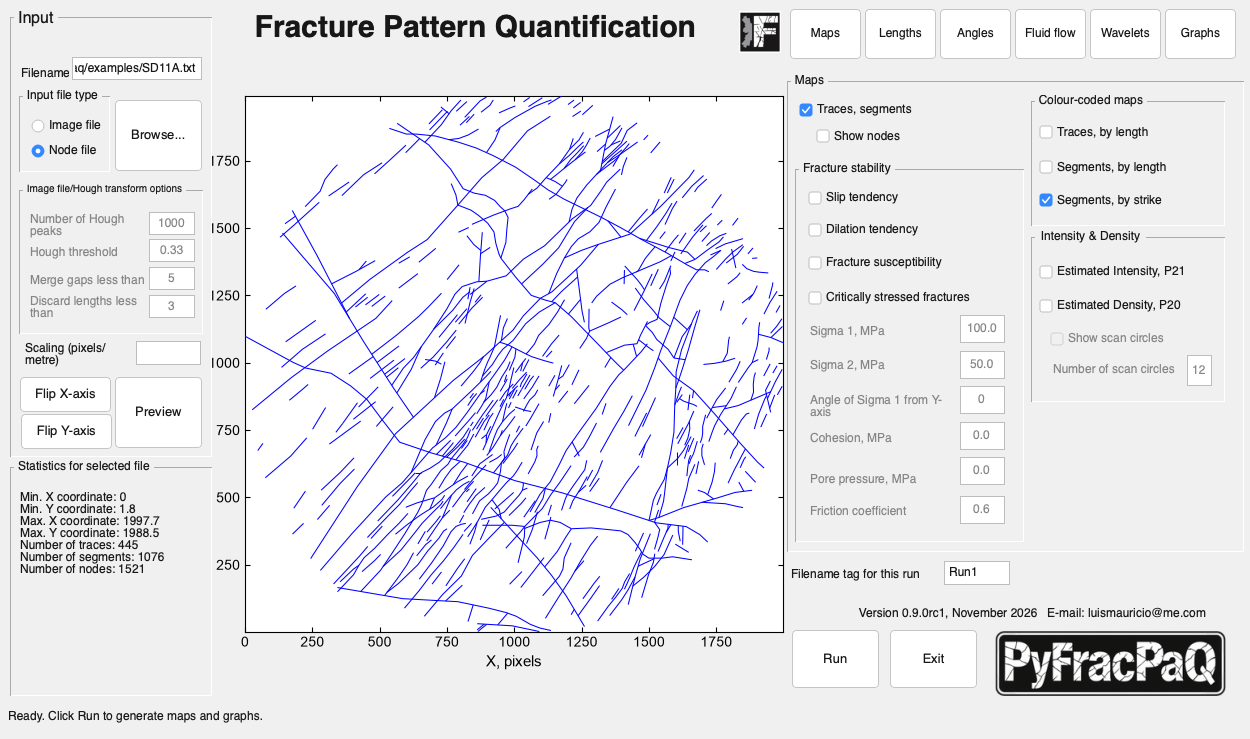
\includegraphics[width=\linewidth]{ui-preview.png}\caption{Actual SD11A preview and statistics. The capture retains the default Run1 tag; use SD11A in the walkthrough to distinguish output files.}\label{fig:preview}\end{figure}

\Needspace{14\baselineskip}
\subsection{Parameters used in this manual's figures}\label{sec:parametros}
The analytical illustrations reuse a reviewed SD11A run with the following parameters, which \emph{are not all GUI defaults}:
\begin{longtable}{@{}p{.43\linewidth}p{.49\linewidth}@{}}
\toprule Group & Illustrated configuration\\\midrule\endhead
Input & No physical scaling or flips; north \(0^\circ\); tag SD11A.\\
Lengths & 20 requested intervals; censoring off; MLE Lower=0 and Upper=0.\\
Angles & 20 requested histogram intervals; \(10^\circ\) rose bins, no length weighting; colour and mean enabled.\\
Maps circular & 12 circles along the shorter side; Show scan circles enabled.\\
Connectivity & 12 blocks; I\(\to\)Y tolerance 2.0 pixels.\\
Stresses & \(\sigma_1=100\), \(\sigma_2=50\) MPa; azimuth \(0^\circ\); cohesion=0, pore pressure=0, friction=0.6. Illustrative values.\\
Permeability & Fixed aperture 0.001 pixel, \(\lambda=1\); no physical calibration.\\
Wavelets & Morlet, a=32, L=2, increment \(90^\circ\). A short demonstration grid.\\
Graphs & Horizontal line from \((0,995.15)\) to \((1997.7,995.15)\); 12 circles.\\\bottomrule
\end{longtable}
Graphs receives points through clicks, rather than coordinate-entry fields. The exact illustrated line was set in the comparison script. An approximate manual selection can change intersections. MLE uses a seed recorded for the illustrated run; the GUI generates its own seeds, so Monte Carlo assessments may vary.

\subsection{States, progress and checking outputs}
Editing the input, scaling, type or Hough parameters invalidates the preview. Run remains disabled until valid geometry is available and while an operation is running. Only parameters needed by the selected analyses are validated. Errors identify the relevant field/tab; choices in other tabs are retained.

Calculations run in the background and figures are presented/exported sequentially through the interface. Wait for completion: MLE and Wavelets can be slow. The main window has no general Cancel button; Exit requests closure at a safe stage. Figures are independent windows with the Matplotlib navigation toolbar. Closing them does not alter the data.

% !TeX root = ../pyfracpaq-user-manual-en.tex
\major{Maps: geometry, sampling and stability}\label{sec:maps}
This tab combines trace/segment maps, attributes, circular sampling and stability. Select only the required options. Show nodes and Show scan circles modify related outputs; they are not independent analyses.
\uifig{ui-maps.png}{The Maps panel. Stability parameters become active when an option in that family is selected.}{fig:ui-maps}

\feature{MAP-01}{Traces, segments and Show nodes}
\textbf{How to use it.} Select \control{Traces, segments}. Enable \control{Show nodes} to draw the input vertices over the traces, then click Run. A polyline represents a mapped fracture; its straight portions are segments, rather than necessarily distinct fractures.

\textbf{Interpretation.} Use this map to identify import problems, isolated traces, excessive segmentation and boundaries. Displaying nodes reveals where a trace has been subdivided. Coincident geometric nodes do not by themselves establish hydraulic connection or a topological class.

\textbf{Output.} One trace map. For SVG inputs containing several colour groups, applicable map selections also add the multicolour map once per Run.
\plotfig{tracemap.png}{SD11A traces with geometric nodes, using the illustrated configuration. The domain remains in pixels.}{fig:traces}

\feature{MAP-04}{Traces, by length}
All segments belonging to a trace receive the colour associated with its total length \(L\). If a fracture was split across several TXT lines, each line has its own length; interpretation therefore depends on digitisation.

Select \control{Traces, by length} and Run. The Lengths histogram need not be selected. Length follows the path, including curved traces. Physical scaling transforms the values before analysis.
\plotfig{tracelengthmap.png}{SD11A coloured by total trace length.}{fig:tracelength}

\feature{MAP-05}{Segments, by length}
Select \control{Segments, by length} to colour each straight portion by its own \(\ell_i\). Compare it with the trace-length map: a long fracture can contain short segments because of its shape or digitisation resolution.

\begin{note}{Colour convention in length maps}
The port retains the approved legacy convention: the colour index is linear in \(L/L_{\max}\), whereas the colourbar is logarithmic. A line's colour must therefore not be interpreted as an exact logarithmic transformation of length. Use the Lengths TXT files for quantitative values.
\end{note}
\plotfig{segmentlengthmap.png}{SD11A coloured by segment length; note the difference from whole-trace length.}{fig:segmentlength}

\feature{MAP-06}{Segments, by strike}
Select \control{Segments, by strike} to map segment orientation. Set \control{Rotate Y-axis from N (°)} in the relevant tab and apply flips to match the data reference. Colour represents corrected axial orientation, not flow direction.

Parallel segments digitised in opposite directions belong to the same axial orientation. Rounding and the representation of zero as \(180^\circ\) in some routines follow the reference convention. Use the histogram/rose to summarise orientation sets, rather than relying solely on the map's visual appearance.
\plotfig{segmentstrikemap.png}{SD11A strike map with north zero and no flips.}{fig:strike}

\subsection{Circular sampling principles}\label{sec:circular}
Sampling uses circular windows within the domain. \control{Number of scan circles} specifies the number along the shorter side, not the total number. The minimum is 2. For shorter extent \(D\) and value \(N\), spacing is \(D/(N+1)\) and \(r=0.99D/[2(N+1)]\); the number along the longer side follows the aspect ratio.

Within each circle, \(n\) counts contacts between finite segments and the circumference, whereas \(m\) counts segment endpoints strictly inside. Tangency contributes once. Events belonging to different segments are counted per segment, so a shared internal vertex can contribute twice to \(m\). A segment wholly inside contributes \(n=0\), while its endpoints contribute to \(m\).
\begin{equation}
\widehat P_{21}=\frac{n}{4r},\qquad
\widehat P_{20}=\frac{m}{2\pi r^2}.
\label{eq:circle}
\end{equation}
Units are length\(^{-1}\) and length\(^{-2}\). These are local estimators affected by sampling, rather than exact measurements of the entire network inside the window. Smaller circles increase spatial resolution and variability; larger circles smooth the comparison.

The console separately reports global measures:
\begin{equation}
P_{21}^{\mathrm{global}}=\frac{\sum_i\ell_i}{A},\qquad
P_{20}^{\mathrm{global}}=\frac{N_{\mathrm{segments}}}{A}.
\end{equation}
They are not averages of the windows. Global density uses \emph{segments}, rather than traces. For unscaled SD11A, the values are approximately 0.01552785 pixel\(^{-1}\) and 0.000271113 pixel\(^{-2}\).

\feature{MAP-07}{Estimated Intensity, P21}
Select the option, enter \(N\) and, to inspect coverage, enable \control{Show scan circles}. Run produces the P21 map; Show scan circles adds a window map shared with P20. Use 12 for the example, giving \(r\simeq75.6474\) pixels.

Hotter colours indicate larger estimator values, not fracture probabilities. Scaling or circle-count changes affect units/resolution; compare maps using consistent parameters. Both intensity and density TXT files are written even if only one map is requested.
\plotfig{intensityP21.png}{Local P21 for SD11A with 12 circles along the shorter side.}{fig:intensity}

\feature{MAP-08}{Estimated Density, P20 and Show scan circles}
Operation follows P21 but uses the second expression in~\eqref{eq:circle}. Inspect the circle map to check observation locations and whether the grid suits the geological scale of interest. All-zero matrices remain zero. A representable display range is assigned to the colourbar without fabricating estimates.

The port uses the approved finite geometric counting in Q-20. A segment is not counted merely because its infinite supporting line intersects the circle outside that segment. This can change legacy results.
\plotfig{densityP20.png}{Local P20 for SD11A. Its inverse-area units and endpoint population differ from P21.}{fig:density}
\plotfig{scancircle.png}{The windows used by the estimators; one circle map is shared by P21/P20.}{fig:scan}

\subsection{Stability map principles}\label{sec:stress}
The four stability selections share parameters. Enter \(\sigma_1\geq\sigma_2>0\) in MPa, the azimuth of \(\sigma_1\), cohesion \(C_0\geq0\), pore pressure \(P_f\geq0\) and friction coefficient \(\mu\geq0\). Compression is positive. Aperture/permeability parameters are not used in this family.

For corrected orientation \(\beta\), stress azimuth \(\psi\) and relative pole \(\alpha=\beta+90^\circ-\psi\),
\begin{align}
\sigma_n&=\left|\frac{\sigma_1+\sigma_2}{2}
+\frac{\sigma_1-\sigma_2}{2}\cos(2\alpha)\right|,\\
|\tau|&=\left|-\frac{\sigma_1-\sigma_2}{2}\sin(2\alpha)\right|.
\label{eq:stress}
\end{align}
Maps use segment orientations. Stability roses evaluate the centres of fixed \(10^\circ\) bins, independently of the bin width in Angles. Each selection generates a map and rose; the family produces one shared Mohr diagram per Run.

\feature{MAP-11}{Slip tendency}
\begin{equation}T_s=\frac{|\tau|}{\sigma_n}.\end{equation}
This is the dimensionless ratio of shear stress to total normal stress. Map/rose colours are normalised by the largest \(T_s\) among corrected segments; the normalised colour is not the physical value of \(T_s\). If the maximum is zero, normalisation remains zero. Comparing colours between samples with different maxima can be misleading.

Select \control{Slip tendency}, enter the stress parameters and Run. This selection also writes segmentdata with raw coordinates/angles; that TXT does not contain \(\sigma_n\), \(\tau\) or \(T_s\).
\plotfig{sliptendencymap.png}{SD11A slip tendency under illustrative stresses, rather than stresses inferred from this sample.}{fig:slip}

\feature{MAP-12}{Dilation tendency}
\begin{equation}T_d=\frac{\sigma_1-\sigma_n}{\sigma_1-\sigma_2}.\end{equation}
Select \control{Dilation tendency}. This describes favourable orientation for dilation under the supplied stress state; it does not calculate actual fracture aperture. It requires \(\sigma_1>\sigma_2\). Equal stresses make the denominator undefined and are rejected for this selection.
\plotfig{dilationtendencymap.png}{Dilation tendency and the spatial distribution of orientations in SD11A.}{fig:dilation}

\feature{MAP-13}{Fracture susceptibility}
\begin{equation}S_f=\sigma_n-P_f-\frac{|\tau|-C_0}{\mu}.\end{equation}
Select \control{Fracture susceptibility}; \(\mu>0\) is required. \(S_f\) has MPa units and expresses the pore-pressure margin in the adopted criterion. Smaller values indicate a smaller margin under the supplied assumptions. The colour scale uses the minimum/maximum of corrected segments. A constant field receives one colour/tick without changing physical values.
\plotfig{fracsuscepmap.png}{SD11A fracture susceptibility with zero cohesion/pore pressure and friction 0.6.}{fig:suscept}

\feature{MAP-14}{Critically stressed fractures}
The classification criterion is
\begin{equation}|\tau|\geq\mu(\sigma_n-P_f)+C_0.\label{eq:csf}\end{equation}
Select \control{Critically stressed fractures}. Equality is included in both map and rose, as approved in Q-17. This is a classification under the chosen stress state, not an observation of active fractures. The illustrative parameters do not justify geomechanical conclusions about the sampling site without independent evidence.
\plotfig{CSFmap.png}{SD11A CSF classification. The count of critically stressed fractures depends on the parameters, not geometry alone.}{fig:csf}

\subsection{Stability roses and the Mohr diagram}
Roses combine orientation frequency with stability evaluated at the bin centre. The \(\sigma_1\) line provides a visual reference. Petal size expresses frequency and colour encodes the indicator; these two quantities must not be confused.
\plotfig{sliptendencyrose.png}{Slip tendency rose: frequency by bin and colour normalised using the observed range.}{fig:stressrose}

The total-stress circle is centred at \((\sigma_1+\sigma_2)/2\) with radius \((\sigma_1-\sigma_2)/2\). For \(P_f>0\), the effective-stress circle shifts the centre by \(-P_f\). The failure envelope is \(\tau=\mu\sigma_n'+C_0\). The port retains the reference framing and does not add individual segment points \((\sigma_n,\tau)\). Their absence does not indicate an import failure.
\plotfig{Mohrplot.png}{The Mohr diagram shared by the stability family. With zero pore pressure, no separate effective-stress circle is drawn.}{fig:mohr}

% !TeX root = ../pyfracpaq-user-manual-en.tex
\major{Lengths: distributions, fits, blocks and variogram}\label{sec:lengths}
This family analyses trace and segment lengths separately. Requested bin settings follow the historical construction of centres: 20 intervals can produce 21 centres. Do not assume that the menu value always equals the final number of bars. The family writes three TXT files even when only the cross-plot, blocks or variogram is selected.
\uifig{ui-lengths.png}{Lengths controls: descriptive statistics, distributions, fits and spatial analyses.}{fig:ui-lengths}

\subsection{Censoring and descriptive statistics}
\control{Censor lengths at map edges} removes a whole trace if its first or last node touches any actual domain boundary. All segments of that trace are removed by the same mask, retaining alignment with their angles. This is a geometric sample selection, rather than a probabilistic correction for unobserved lengths.

An internal vertex touching a boundary is not automatically a censored endpoint. The domain is defined before selection. If censoring removes everything, the run is rejected before the family's files are written, preserving existing files. Leave censoring off to reproduce the SD11A figures.

The console reports count, minimum, maximum and arithmetic mean, \(\bar L=N^{-1}\sum_i L_i\), for both populations. Without censoring, the example gives:
\begin{center}\begin{tabular}{@{}lrrrr@{}}\toprule
Population & N & Minimum & Maximum & Mean\\\midrule
Traces &445&7.42496&2057.12077&138.48854\\
Segments &1076&6.32851&318.36999&57.27454\\\bottomrule
\end{tabular}\end{center}
Lengths are in pixels. Different means are expected because the number of segments per trace varies.

\feature{LEN-02}{Histogram of lengths}
Select \control{Histogram of lengths} and choose the bin setting. Run produces two figures: trace and segment lengths, each with absolute frequency and the corresponding percentage axis. For a bin containing \(n_j\) observations, the percentage is \(100n_j/N\).

Use the histograms to compare populations and identify common lengths without mistaking histogram shape for a statistical model. More bins reduce observations per bin and can make the extremes less stable. If all lengths are equal, one populated bin is used without artificial jitter.
\plotfig{histotracelength.png}{The SD11A trace-length histogram, rather than the distribution of all segments.}{fig:lengthhist}
\plotfig{histosegmentlength.png}{The SD11A segment-length histogram. Subdivision shifts the population towards shorter lengths.}{fig:segmenthist}

\feature{LEN-03}{Log-log lengths}
Select \control{Log-log lengths}. Four figures are produced: binned frequencies and complementary frequencies for each population. Both axes are logarithmic; zero-frequency points are not plotted.

Conceptually, complementary frequency describes observations above a length. The implementation retains the legacy construction:
\begin{equation}
C_j=N-\sum_{k\leq j} n_k,
\end{equation}
where \(n_k\) are counted around bin centres. The complementary grid has unit spacing in pixels and 1000 intervals (1001 centres) in metres, except for a constant sample. It is therefore not an unbinned empirical function evaluated at every observed length.

Figures called \emph{density distribution} show histogram frequencies on log-log axes, rather than a probability density normalised by bin width. An approximately straight pattern does not establish a power law. Consider MLE, sampling and censoring together.

The red vertical line in the complementary plot represents the domain diagonal rounded upwards. It is a geometric reference, not an imposed upper bound on the path length of a curved trace, which may exceed it.
\plotfig{loglogplottracelength.png}{Complementary trace-length frequencies. Positive points are displayed on log-log axes.}{fig:loglog}
\plotfig{loglogplotsegmentlengthdensity.png}{Binned segment frequencies on log-log axes, not normalised probabilities.}{fig:logdensity}

\feature{LEN-06}{Cross-plot lengths v angles}
Select \control{Cross-plot lengths v angles}; it can run on its own. Each observation pairs segment length with corrected orientation, using axial duplication for the angular display. It does not pair whole-trace length with a mean trace angle.

Check whether longer segments concentrate in particular orientation sets, considering digitisation effects. North/flips follow this family's angular convention. Historical plotting limits can omit values that legacy angular correction leaves outside the displayed interval; diagnostics and preserved data distinguish that from import loss.
\plotfig{crossplotsegmentlengthangle.png}{SD11A cross-plot showing the association between segment orientation and length.}{fig:cross}

\feature{LEN-07}{MLE analysis: three models and two populations}\label{sec:mle}
Enable \control{Log-log lengths}, then \control{MLE analysis}. Enter Lower/Upper percentage cut-offs; use zero for both in this walkthrough. Lower removes the \(\lceil Np_{\mathrm{lower}}/100\rceil\) smallest observations and Upper the \(\lceil Np_{\mathrm{upper}}/100\rceil\) largest after sorting. These are percentages of observations, not length thresholds in the axis unit.

The same retained population is used for searching and final fitting, as approved in Q-15. For each model, candidate lower bounds \(x_{\min}\) are tested. The tail minimising the distance between complementary curves is selected, with at least two observations and two distinct values. Ties favour the smaller \(x_{\min}\). Not every observed length must belong to the fitted tail.

For \(z_i\geq x_{\min}\), the adopted estimators are
\begin{align}
\widehat\alpha&=1+\frac{n}{\sum_i\ln(z_i/x_{\min})}
&&\text{(power law)},\\
\widehat\lambda&=\frac{1}{\overline{z-x_{\min}}}
&&\text{(exponential)},\\
\widehat\mu&=\frac1n\sum_i\ln z_i,\qquad
\widehat\sigma^2=\frac1n\sum_i(\ln z_i-\widehat\mu)^2
&&\text{(lognormal)}.
\end{align}
\(\alpha\) and \(\sigma\) are dimensionless; \(\lambda\) has inverse-length units and \(\mu\) depends on the logarithm of the chosen length unit. The lognormal estimator uses the mean and deviation of tail log-lengths, following the supplied implementation. It is not a new optimisation of a conditionally truncated lognormal distribution.

The curves used are
\begin{align}
S_{\mathrm{PL}}(x)&=(x/x_{\min})^{1-\alpha},\\
S_{\mathrm{Exp}}(x)&=\exp[-\lambda(x-x_{\min})],\\
S_{\mathrm{LN}}(x)&=\Phi\!\left(-\frac{\ln x-\mu}{\sigma}\right),
\end{align}
where \(\Phi\) is the standard normal distribution function. Figures retain FracPaQ's scaling and display conventions. Power-law fits use log-log axes, exponential fits linear-log and lognormal fits log-linear; check the axes before comparing curvature.

\textbf{Outputs.} Six fitted-model figures: three for traces and three for segments. The Log-log selection also produces its four figures, without recalculating the family or duplicating TXT files. Parameter boxes show estimates and assessments; cut-off lines help identify the population.
\plotfig{tracelengthsFittingPowerLaw.png}{Example power-law MLE fit to SD11A trace lengths. Do not extrapolate beyond the tail without justification.}{fig:mlepl}
\plotfig{tracelengthsFittingExponential.png}{Example exponential fit to traces; axis scaling differs from the power-law figure.}{fig:mleexp}
\plotfig{tracelengthsFittingLogNormal.png}{Example lognormal fit to traces. The same analysis is performed separately for segments.}{fig:mleln}

\subsubsection{Interpreting the tests and rates}
The Kolmogorov--Smirnov distance compares the two empirical step functions:
\begin{equation}D=\sup_x|F_1(x)-F_2(x)|.\end{equation}
The procedure retains 2500 two-sample comparisons per model, an asymptotic p-value and a two-sided hypothesis. Decisions use \(p\leq\alpha_{\mathrm{sig}}\), with significance 0.1 for the power law and 0.05 for exponential/lognormal models. Another rate counts \(p>0.05\) for all three models. These quantities do not share the same definition.

\begin{note}{Statistical interpretation}
The rates are not posterior probabilities that a model is true. Failure to reject does not prove the distribution, and a straight log-log pattern does not identify it. The six assessments use Monte Carlo: the GUI records a seed and independent runs may vary. This manual's figures come from a comparison run with a recorded seed. See Clauset et al.~\cite{clauset} for general background; the implemented procedure retains the FracPaQ-specific choices described here.
\end{note}

\feature{LEN-13}{Block size graphs}
Select \control{Block size graphs}. The network is rasterised in the original coordinate system with a defined trace thickness. White components with eight-connectivity touching the border are excluded; the remaining components represent closed blocks in the raster. Outputs include a centroid map, area histogram and complementary log-log plot, plus a fixed-name BMP.

If a component contains \(n_p\) pixels and each pixel represents \(\Delta x\Delta y\),
\begin{equation}A_b=n_p\Delta x\Delta y.\end{equation}
Centroids are calculated from pixel centres. Resolution remains in the original coordinates when physical scaling is applied; areas change by \(1/s^2\) and centres by \(1/s\). Trace ink occupies area, so this is not exact vector-polygon area. Small closures, gaps and resolution can change the block count.

The illustrated SD11A configuration yields 67 accepted components. This excludes the exterior and is not a three-dimensional block count. If no closed component exists, figures state that rather than fabricating areas. Also inspect \code{examples/rectangles.txt}: each rasterised interior of a 40-by-40 square has area 1444 pixels\(^{2}\), rather than 1600, because of trace ink.
\plotfig{blocksizecentroidmap.png}{Centroids of the blocks identified in the SD11A raster.}{fig:blocks}
\plotfig{blocksizehisto.png}{Area distribution of accepted components. The intermediate BMP supports checking the segmentation.}{fig:blockhist}

\feature{LEN-15}{Variogram of segment lengths}
Select \control{Variogram of segment lengths}. Positions are segment centres and values are their lengths, after the common censoring mask when enabled. The experimental semivariogram for a distance bin is
\begin{equation}
\widehat\gamma(h)=\frac{1}{2N(h)}\sum_{(i,j)\in h}(\ell_i-\ell_j)^2.
\end{equation}
Distance has length units and \(\gamma\) length-squared units. Similar nearby segments tend to give smaller differences, but trends, orientation and sampling design also influence the curve.

The GUI uses 30 bins and a maximum distance of half the diagonal of the segment-centre envelope. Empty bins have no estimate. The GUI does not fit a theoretical model or calculate kriging, range or nugget parameters. The historical pair convention includes the diagonal below 1000 observations and excludes it from 1000 onwards; SD11A contains 1076 segments. Do not compare populations without accounting for that convention.
\plotfig{segmentlength_variogram.png}{Experimental SD11A segment-length semivariogram, with no theoretical curve fitted.}{fig:variogram}

\major{Angles: histograms and rose diagrams}\label{sec:angles}
The data are axial: opposite orientations represent the same fracture direction. Circular display duplicates each orientation by \(180^\circ\), then applies the relevant angular conventions. This does not double the physical number of segments.
\uifig{ui-angles.png}{Angles controls: north, histogram, petal width and display options.}{fig:ui-angles}

\feature{ANG-01}{Histogram of angles}
Select \control{Histogram of angles} and choose 10, 20, 30 or 50 requested intervals. The historical construction uses centres from 0 to \(360^\circ\), potentially giving one more centre than the menu value. The axis represents orientation, not the network's X/Y position.

Frequency counts segments, with axial duplication for display. If legacy angular correction leaves values outside \([0,360]\), the application reports that case. Histogram and rose behaviour is retained instead of silently introducing a new normalisation. Compare samples using the same north, flips and bin settings.
\plotfig{histoangle.png}{SD11A angle histogram with north zero. Compare frequencies within the same axial convention.}{fig:anglehist}

\feature{ANG-02}{Rose diagram (equal area)}
Select \control{Rose diagram (equal area)} and a petal width of 5, 10, 20 or \(30^\circ\). The default contribution is segment count. \control{Length weighted?} uses length as weight; \control{Colour by strike?} changes colour presentation and \control{Show mean vector?} adds the mean reference when selected.

For bin percentage \(p_j\), radius is proportional to its square root:
\begin{equation}r_j=50\sqrt{p_j}.\end{equation}
Petal area is therefore proportional to percentage; radius is not the percentage itself. With weighting, the contribution follows the sum of bin lengths divided by total length. Bins across the 0/180/360 seam retain FracPaQ's historical adjustments; this is not a generic polar histogram.

Axial statistics use doubled angles:
\begin{align}
C&=\frac1N\sum_i\cos(2\beta_i),\quad
S=\frac1N\sum_i\sin(2\beta_i),\quad R=\sqrt{C^2+S^2},\\
\overline\beta&=\frac12\operatorname{atan2}(S,C),\qquad
s_\beta=\sqrt{2(1-R)}.
\end{align}
The \(s_\beta\) expression is in radians and is converted to degrees by the application. The mean is adjusted to the axial representation. These statistics are unweighted in the implementation even when the rose is length weighted. \(R\) near zero indicates no dominant mean orientation; do not treat a plotted mean line as a robust structural direction in that case.
\plotfig{roseangleEqArea.png}{Unweighted SD11A rose with 10-degree petals. Radius grows with the square root of percentage.}{fig:rose}

% !TeX root = ../pyfracpaq-user-manual-en.tex
\major{Fluid flow: topology, crack tensors and permeability}\label{sec:flow}
These three features describe different aspects of the network. An I/Y/X diagram is not a hydraulic solution, and the permeability factor \(\lambda\) is not automatically calculated from it.
\uifig{ui-fluid.png}{Fluid flow controls: topological classification, tensors and aperture settings for permeability estimation.}{fig:ui-fluid}

\feature{FLO-01}{I-Y-X connectivity}
Select \control{I-Y-X connectivity}. Enter \control{Number of blocks in maps} (integer \(\geq2\)) and \control{Distance to count I as Y} (\(\geq0\), in the current length unit). Use 12 and 2.0 pixels for the illustrated SD11A example.

Classification follows encounters between traces, rather than simply counting TXT vertices:
\begin{itemize}
\item \textbf{I}: an isolated endpoint with one branch.
\item \textbf{Y}: a three-branch junction, including an exact T and a real endpoint close to another segment within the tolerance.
\item \textbf{X}: a four-branch crossing in the adopted model.
\end{itemize}
Proximity is Euclidean and inclusive, measured to a finite segment of another trace. An undershoot may produce an inferred Y. An internal vertex is not an endpoint. An exact T is Y even at zero tolerance. Original geometry is not rewritten to perform classification. Collinear overlaps and self-intersections do not automatically constitute inter-trace junctions.

Triangle fractions are
\begin{equation}f_I=\frac{N_I}{N_I+N_Y+N_X},\quad f_Y=\frac{N_Y}{N_I+N_Y+N_X},\quad f_X=\frac{N_X}{N_I+N_Y+N_X}.
\end{equation}
The triangle summarises proportions, but spatially different networks may share those fractions. Sanderson and Nixon~\cite{sanderson} discuss the topological framework; the port's specific proximity rules are those stated above.

Run produces four figures: an I/Y/X node map, an X+Y heatmap, an I heatmap and the triangle, plus one TXT. Under the illustrated settings, SD11A has \(N_I=606\), \(N_Y=224\), \(N_X=90\). TXT rows retain the order I, X, Y; do not swap the last two classes when reading it.
\plotfig{IYXnodes_traces.png}{SD11A node classification. Counts depend on tolerance and digitisation.}{fig:iyxnodes}
\plotfig{IYXtriangle.png}{The SD11A topology triangle. Square/circular markers use ordinary geometric shapes.}{fig:triangle}

Heatmaps show \emph{counts} per block, rather than area-normalised densities. The block count along the longer side follows the aspect ratio. The historical bin construction uses the coordinate range of each non-empty class, so the maps do not necessarily represent identical spatial cells. Absent classes are handled without fabricating nodes.
\plotfig{XYnodes_traces_heat.png}{Spatial X+Y node counts, useful for locating concentrations of junctions.}{fig:xyheat}

\feature{FLO-08}{Crack tensor plot}
Select \control{Crack tensor plot}. For segment \(i\), length \(\ell_i\), unit normal \(\mathbf n_i\) and node-envelope area \(A\), define
\begin{equation}
F^{(0)}=\sum_i\frac{\ell_i^2}{A},\qquad
\mathbf F^{(m)}=\sum_i\frac{\ell_i^2}{A}\,\mathbf n_i^{\otimes m},
\quad m=2,4,8.
\end{equation}
The projection plotted in direction \(\mathbf v\) is
\(F_m(\mathbf v)=\sum_i(\ell_i^2/A)(\mathbf n_i\cdot\mathbf v)^m\).
These are angular descriptors weighted by squared length. Higher orders emphasise directional variation differently; they do not represent additional spatial dimensions of the outcrop.

Run produces one figure containing orders 0/2/4/8 and also triggers EZROSE because it uses the angular family. The envelope requires positive area, including for networks extracted from images; a single line cannot support this calculation. Poles use the reference's own north, rounding and flip convention.
\plotfig{cracktensor.png}{SD11A crack tensor projections. The order-zero curve provides an isotropic reference for the weight.}{fig:crack}

\feature{FLO-09}{Permeability plot (polar)}
Select \control{Permeability plot (polar)}. Choose a fixed aperture \(t\geq0\), or scaled apertures \(t_i=a\ell_i^b\), with factor \(0\leq a\leq0.1\), exponent \(0.5\leq b\leq1\) and \(0\leq\lambda\leq1\). Only parameters belonging to the active mode are used.

The adopted parallel-plate model calculates
\begin{align}
\mathbf P&=\sum_i\frac{t_i^3\ell_i}{A}\,\mathbf n_i\otimes\mathbf n_i,\\
\mathbf K&=\frac{\lambda}{12}\left[\operatorname{tr}(\mathbf P)\mathbf I-\mathbf P\right],\qquad
k(\mathbf v)=\mathbf v^{\!T}\mathbf K\mathbf v.
\end{align}
Area refers to the node envelope, not automatically the whole image. The polar curve is a directional projection; eigenvalues give principal maxima/minima. \(\mathbf K\) has area units. Without physical calibration, results are in pixel\(^{2}\), not physical permeability in m\(^{2}\).

Doubling aperture multiplies \(\mathbf K\) by eight; \(\lambda\) acts linearly. Zero aperture or \(\lambda=0\) gives the zero tensor. \control{Lambda factor} is a user choice independent of I/Y/X counts. Enter aperture in the current length unit: scaling does not automatically convert its numerical input. For scaled apertures, the unit of \(a\) depends on \(b\).

In the unscaled example with fixed aperture 0.001 pixel and \(\lambda=1\), eigenvalues are approximately \(2.8756\times10^{-13}\) and \(1.00643\times10^{-12}\) pixel\(^{2}\). These illustrate the calculation, rather than estimating physical material properties. This option produces a PNG and console messages, without its own new TXT.
\plotfig{permeability_polar.png}{SD11A polar permeability projection under illustrative aperture and \(\lambda\) settings.}{fig:permeability}

\major{Wavelets 2D: scale, orientation and anisotropy}\label{sec:wavelets}
\feature{WAV-01}{Run wavelet analysis}
The analysis searches for oriented structures at different scales in a network raster. Select \control{Run wavelet analysis}, choose Morlet or Mexican Hat and enter lists of a, L and an angular increment.
\uifig{ui-wavelets.png}{The Wavelets panel. Lists contain space-separated numbers, not MATLAB expressions.}{fig:ui-wavelets}

\subsubsection{Parameters and a first run}
Use \(a=32\), \(L=2\) and a \(90^\circ\) increment to follow this manual's figure. This is a short demonstration, not a research-resolution recommendation. A finer grid might use a=16 32, L=2 4 and an increment of 30, at greater cost.

The a/L lists require positive, space-separated integers: enter \code{8 16 32}, not \code{8:8:32}. The increment must be a positive integer divisor of \(180^\circ\), such as 10, 20, 30, 45, 60 or 90. The calculation uses anisotropy ratio \(r=1/L\). L=1 is isotropic and may give a physically indeterminate orientation in a tie.

\subsubsection{Raster and kernels}
The raster retains the 27-inch, 72-dpi contract: 1944\(\times\)1944 pixels with defined margins and line widths. Traces at least 45\% as long as the longest use 4 points; other traces use 1. White becomes zero background through normalisation. Physical scaling and north are not inserted into raster coordinates.

For centred coordinates rotated and divided by a, \((\xi,\eta)\), and \(q=(r\xi)^2+\eta^2\), the implemented kernels have the forms
\begin{align}
\psi_M&=\frac{\sqrt r}{a}\exp(-2\pi\mathrm i\eta)\exp(-q/2),\\
\psi_H&=\frac{2-q}{a}\exp(-q/2).
\end{align}
The response is the discrete convolution of the demeaned image with the real kernel, calculated by FFT and cropped to the original dimensions. For Morlet, the kernel's self-response retains the complex term; it is not replaced by magnitude squared.

The normalisation used in selection is
\begin{equation}
WC(a,\theta,L)=\frac{2.5\,|W|}{a\,\max|W_{\mathrm{self}}|}.
\end{equation}
At each position and a, the maximum WC over orientations and factors is retained. Numerical orientation ties use the first stable choice, as approved in Q-12. Recorded energy is the sum of squared response values. This describes the port's implementation, rather than claiming equivalence between all CWT definitions in the literature.

\subsubsection{Reading the panels and files}
Each a produces a 2\(\times\)2 panel: input raster, WC map, a rose of selected orientations and a histogram of \(\log_{10}\) frequency. The mask is fixed and strict:
\begin{equation}WC>0.5\,\max(WC).
\end{equation}
There is no threshold slider. The optimum raster orientation is converted to the rose's axial representation. North is not used, and flips follow this family's convention.

Each a also writes a theta TXT. The intermediate raster has a fixed, untagged name. Work grows approximately with the product of the numbers of a, L and orientations, as well as FFT size. The application estimates memory and limits this family to a 2-GiB working budget; reducing the grid may be necessary. Input TXT size is not a useful predictor of Wavelet cost.
\plotfig{wavelet_a32.png}{SD11A with Morlet, a=32, L=2 and a 90-degree angular step. The coarse sampling is illustrative; the WC colourbar is not a probability scale.}{fig:wavelet}

\major{Graphs: ALONG and FROM profiles}\label{sec:graphs}
First select a line in the preview. Click \control{Select end points}, then two distinct points inside the map in the desired order. Escape or right-click cancels the attempt while preserving the last complete line. A coincident second point must be chosen again. Clicks outside the axes are ignored; Run is disabled during an incomplete selection.
\uifig{ui-graphs.png}{Graphs combines line selection and profiles. P21/P20 share the circles along that line.}{fig:ui-graphs}

Changing input, scaling, type or Hough parameters, or making a new preview, clears the line; flips and north preserve it. The illustrated line runs from \((0,995.15)\) to \((1997.7,995.15)\). Points are selected by clicks in the GUI, so small differences are expected.

\subsection{Geometric definitions}
For endpoints \(\mathbf p_1\), \(\mathbf p_2\), vector \(\mathbf d=(d_x,d_y)=\mathbf p_2-\mathbf p_1\) and \(D=\|\mathbf d\|\), ALONG uses the finite line and distance from the intersection to point 1. FROM uses the infinite line and signed distance from a point \((x,y)\):
\begin{equation}
d_\perp=\frac{d_y(x-x_1)-d_x(y-y_1)}{D}.
\end{equation}
For a horizontal line running left to right, points above it have negative distance. Reversing the line reverses the FROM sign and changes the ALONG origin. North and flips do not correct the raw angles in these profiles; flips affect their auxiliary map.

ALONG retains one record per intersecting segment. A curved trace may appear several times and a shared vertex can yield two observations. Collinear contacts are excluded. Results are not automatically sorted or deduplicated. If no intersections exist, ALONG profiles state that without blocking the other analyses.

\feature{GRA-03}{ALONG: Trace length}
Select the option after choosing a line. At each encounter, Y is the total length of the corresponding trace and X is distance from point 1. Repeated intersections with a single trace may repeat the same length; this is not duplication of the input TXT.
\plotfig{tracelengthalonggraph.png}{Total lengths of traces intersecting the SD11A profile line.}{fig:tracealong}

\feature{GRA-04}{ALONG: Segment length}
The same intersections are used, but Y is the encountered segment's length, rather than whole-trace length. Compare this profile with the previous one to see where long traces have been subdivided.
\plotfig{segmentlengthalonggraph.png}{Lengths of segments intersected by the profile line.}{fig:segmentalong}

\feature{GRA-05}{ALONG: Segment angle}
This plots raw segment angle at each intersection. Clusters can suggest changing orientation sets along the line; the profile is not a local rose or a window-averaged angle.
\plotfig{segmentanglealonggraph.png}{Raw segment angles along the SD11A profile.}{fig:anglealong}

\feature{GRA-06}{ALONG: Estimated intensity, P21}
Choose an integer \control{Number of scan circles} \(\geq2\). Here, \(r=D/(2N)\), centres occur at fractions \((k+0.5)/N\) along the line and abscissae run from r to \(D-r\). This differs from the rectangular Maps grid. The estimator is \(n/(4r)\), using the finite counting rules already described.

Selecting either P21 or P20 produces the circle map and both profiles once per Run. Inspect the map for coverage. The map identifies Point 1/Point 2 with the corresponding marker colours.
\plotfig{graphtracemap.png}{The SD11A profile line and circles. Radius depends on line length and N.}{fig:graphmap}
\plotfig{intensityalonggraph.png}{Estimated intensity along the profile with 12 circles.}{fig:graphintensity}

\feature{GRA-07}{ALONG: Estimated density, P20}
This uses the same circles and \(m/(2\pi r^2)\). Squaring the radius is the approved Q-20 correction; the legacy Graphs denominator linear in r was not retained. Units are inverse area, consistent with Maps. P21 and P20 count different events, rather than expressing the same quantity at different scales.
\plotfig{densityalonggraph.png}{Estimated density along the same profile, with the approved area normalisation.}{fig:graphdensity}

\feature{GRA-10}{FROM: Trace length}
Each trace contributes its halfway-along-path centre and total length. X is the signed centre-to-infinite-line distance; intersection with the finite profile is unnecessary. This is not the nearest-endpoint distance or the mean distance of its vertices.
\plotfig{tracelengthfromgraph.png}{Trace lengths against signed distance from their centres to the reference line.}{fig:tracefrom}

\feature{GRA-11}{FROM: Segment length}
Each segment contributes its geometric centre and length. A trace may appear at several distances because it contains several segments. The infinite line supports comparing its two sides but does not define a finite-width sampling strip.
\plotfig{segmentlengthfromgraph.png}{Segment lengths against signed distance to the reference line.}{fig:segmentfrom}

\feature{GRA-12}{FROM: Segment angle}
This uses segment centres and their raw angles. Observe the sign convention when comparing sides: reversing the line reverses the sign. Graphs produces PNGs without a dedicated profile TXT.
\plotfig{segmentanglefromgraph.png}{Segment orientations on both sides of the SD11A reference line.}{fig:anglefrom}

% !TeX root = ../pyfracpaq-user-manual-en.tex
\major{Complementary tools}\label{sec:aux}
Use the same prepared Python executable from the project root. With Miniforge activated, replace \code{.venv/bin/python} with \code{python}. Quote paths containing spaces.

\subsection{Preprocess photographs for Hough}
\begin{verbatim}
.venv/bin/python -m pyfracpaq.tools preprocess photo.jpg \
  prepared.tif --panel stages.png
\end{verbatim}
The command accepts eight-bit RGB/grayscale input and requires distinct paths for the input, TIFF and PNG panel. The TIFF is a binary 0/255 grayscale image. Grayscale conversion approximates \(0.298936R+0.587043G+0.114021B\), with rounding. The median uses a 20\(\times\)20 window; saturated subtraction is
\begin{equation}D=\max\{\operatorname{median}(I)-I,0\}.\end{equation}
Sobel, morphological closing and thinning/inversion follow. The median estimates the background, subtraction highlights dark structures and Sobel responds to gradients. Closing/thinning changes connectivity and thickness, potentially joining or losing traces. Inspect the panel before import. There is no AI segmentation.
\plotfig{preprocess.png}{Preprocessing a reference photograph, separate from SD11A and the Hough example.}{fig:preprocess}

\subsection{Convert Move objects to nodes}
\begin{verbatim}
.venv/bin/python -m pyfracpaq.tools move \
  examples/move_objects.dat nodes.txt \
  --x-column 1 --y-column 3 --skip-header 1
\end{verbatim}
Columns are one-based; defaults are X=1, Y=3 and no header lines. The supplied example requires one header line. Blank lines separate objects and the last object is retained even without a final blank line. TXT output uses four decimal places and TAB. Check it in Preview. A conversion error does not replace the previous output file.

\subsection{Wavelet dialogue for an existing raster}
\begin{verbatim}
.venv/bin/python -m pyfracpaq.tools wavelet-dialog \
  FracPaQ2D_wavelet_traces.png \
  --output-directory . --tag Run1
\end{verbatim}
The dialogue accepts eight-bit L/RGB rasters and reuses the kernels/parameters in Section~\ref{sec:wavelets}. Run freezes its configuration and processes its own job. Cancel requests interruption at a safe stage or closes only the dialogue. The main preview is not replaced. PNGs use the tool's tag, but theta TXT retains the auxiliary \emph{untagged} filename. Changing --tag alone does not separate those TXT files.

\subsection{APIs and legacy resources}
An advanced variogram, order-16 tensor, linear/historical roses, probePlane, generic text reader and palettes are also available through Python APIs. They are not extra GUI 2.8 controls. Incomplete experiments and earlier interfaces remain references without new buttons. Their contracts are in the development documentation; ordinary tab use does not depend on them.

\major{Output files and organisation}\label{sec:exports}
\subsection{Figures, tags and output counts}
Analytical PNGs use 20\(\times\)20 cm at 600 dpi, or 4724\(\times\)4724 pixels in the checked backend. Window size does not change that export resolution. Horizontal colourbars track plot width and vertical colourbars plot height, maintaining fixed clearance from axis labels.

Most filenames follow \code{FracPaQ2D_name_SD11A.png}, where name stands for the output name. Graphs uses \code{guiFracPaQ2D_}; Wavelets uses, for example, \code{FracPaQ2Dwavelet_a32_SD11A.png}. The underscore before the tag remains when the tag is empty. Spaces/accents are accepted; path separators and reserved characters are rejected. A tag does not select a folder.
\begin{longtable}{@{}p{.29\linewidth}p{.63\linewidth}@{}}
\toprule Selection & PNGs per Run\\\midrule\endhead
Traces/length/strike & One per selection; SVG may add a multicolour map.\\
P21/P20 in Maps & One per map; Show scan circles adds a shared circle map.\\
Stability & Map and rose per selection; one Mohr diagram per family.\\
Lengths histograms & Two: traces and segments.\\
Log-log lengths & Four: binned frequencies and complementary frequencies for both populations.\\
MLE & Six additional figures, three models per population.\\
Cross-plot/variogram & One per selection.\\
Blocks & Three: centroids, histogram and complementary distribution.\\
Angle histogram/rose & One per selection.\\
I-Y-X & Four: nodes, X+Y heatmap, I heatmap and triangle.\\
Tensors/permeability & One per selection.\\
Wavelets & One panel per a, plus the fixed raster.\\
Graphs & One per attribute profile; P21/P20 share a map and both circular profiles.\\
Image Preview & Hough diagnostic before Run.\\\bottomrule
\end{longtable}
The default Run produces five PNGs and four TXT files. One checkbox does not necessarily correspond to one file.

\subsection{TXT and intermediate files}\label{sec:txt}
The names below use tag SD11A and a=32. TXT files have no header, apart from the connectivity class letters.
\begin{longtable}{@{}p{.54\linewidth}p{.38\linewidth}@{}}
\toprule File & Content\\\midrule\endhead
\code{FracPaQ2Dsegmentlengths_SD11A.txt} & Sorted segment lengths; two decimal places.\\
\code{FracPaQ2Dtracelengths_SD11A.txt} & Sorted trace lengths; two decimal places.\\
\code{FracPaQ2Dsegmentangleslengths_SD11A.txt} & Raw angle/length pairs, aligned in source order; two decimal places.\\
\code{FracPaQ2DEZROSE_SD11A.txt} & Corrected, axially duplicated and sorted angles; two decimal places.\\
\code{FracPaQ2Dintensity_SD11A.txt} & X/Y/P21; centres to one decimal place, estimate to eight.\\
\code{FracPaQ2Ddensity_SD11A.txt} & X/Y/P20, X outer/Y inner traversal.\\
\code{FracPaQ2Dconnectivity_SD11A.txt} & Rows I, X and Y with their counts.\\
\code{FracPaQ2Dsegmentdata_SD11A.txt} & One-based sequence, X1/Y1/X2/Y2 to four decimal places and raw angle to one.\\
\code{FracPaQ2Dwavelet_theta_a32_SD11A.txt} & Main-tab selected orientations, one per line.\\
\code{name_converted.txt} /\newline\code{name_colourHHHHHH_converted.txt} & SVG nodes beside the source, grouped by colour where required.\\
\code{FracPaQ2D_blocksize.bmp} & Block raster, fixed and untagged.\\
\code{FracPaQ2D_wavelet_traces.png} & 72-dpi Wavelet raster, fixed and untagged.\\
\code{FracPaQ2Dwavelet_theta_a32.txt} & Auxiliary dialogue theta, untagged.\\\bottomrule
\end{longtable}
Lengths writes its three TXT files whenever that family is selected. Angles/crack tensor triggers EZROSE. P21 or P20 in Maps writes both circular TXT files. Only Slip tendency writes segmentdata. Graphs has no dedicated TXT. Preprocess writes to the supplied paths, and its panel resolution differs from the analytical PNG resolution.

The historical text precision rounds values: different centres may appear identical in small units. Internal arrays retain their precision. Statistical tables are not node TXT files and should not be imported as such.

\subsection{Replacement and partial runs}
Each file is prepared in its own temporary file and atomically replaced. There is no single transaction covering a whole Run. A failure/interruption may leave files from different runs together; inspect the messages and folder. An error does not automatically roll back every file, and no generic cleanup of unrelated files is performed.

\major{Interpretation and troubleshooting}\label{sec:limites}
\subsection{A sequence for responsible analysis}
\begin{enumerate}
\item Check geometry/statistics and decide calibration before interpreting units.
\item Compare maps against histograms/roses; assess segmentation and the angular reference.
\item Try justified P21/P20 resolutions and record N/radius.
\item Justify topological tolerance from digitisation, rather than the desired triangle appearance.
\item Decide censoring before tail fitting; record cut-offs and parameters.
\item Orient profiles around a geological question; state their points, direction and units.
\item Interpret permeability/stability physically only with independently justified aperture/stress data.
\item For Wavelets, state the raster, a, L and angular increment.
\end{enumerate}

\subsection{Approved differences}
Q-05 applies trace-level censoring; Q-11 uses real-endpoint proximity. Q-12 defines the Wavelet raster, dimensions and tie handling. Q-14 excludes the exterior and calibrates blocks. Q-15 corrects cut-offs and tail searches. Q-17 corrects normalisation, colours and CSF equality. Q-20 uses finite counting and area-normalised P20. These are active defaults and may differ from legacy results.

Raw/corrected angular conventions and linear colour indices with logarithmic colourbars in length maps are retained. Visual differences in five titles and two Hough side views were accepted without authorising changes to accumulators, peaks or endpoints. Markers use ordinary squares/circles. This does not establish universal pixel identity, equivalence to corrected legacy scientific results or suitability for every sample. Detailed audits are optional material in the full clone.

\Needspace{27\baselineskip}
\subsection{Common diagnostics}
\begin{longtable}{@{}p{.34\linewidth}p{.58\linewidth}@{}}
\toprule Situation & Check\\\midrule\endhead
Run disabled & Refresh the preview; wait for processing; complete/cancel profile-line selection.\\
TXT rejected & TABs, complete pairs, no header, finite values and two distinct nodes per trace.\\
SVG rejected & Prepare curves, transforms and CSS in the source editor; do not merely change the extension.\\
Image rejected & Eight-bit grayscale, JPEG/TIFF, single frame; RGB/alpha requires preparation.\\
Hough finds no lines & Check white/background, threshold, FillGap and MinLength in the diagnostic.\\
Tensor/circular Maps fails & Check that the two-dimensional area is positive.\\
MLE has no sample & Recheck censoring/cut-offs; the tail needs two distinct values.\\
No blocks & Check closures, trace ink and raster resolution in the BMP.\\
ALONG is empty & The finite line must meet non-collinear segments; FROM uses different geometry.\\
Wavelets is slow & Reduce a, L and orientations; respect the memory budget.\\
Permeability in pixel\(^{2}\) & Physical calibration is missing; do not relabel the axis as metres.\\
ModuleNotFoundError & Check the interpreter, project root and requirements.txt installation with the same Python.\\\bottomrule
\end{longtable}

\subsection{Minimum record for reproducibility}
Keep the input/checksum, version, scale/units, north/flips, selections, bins, censoring/cut-offs, tolerance, physical parameters, profile points, Wavelet grid, tag and folder. For Monte Carlo, also retain the console seed. The GUI does not save a complete session; a PNG alone does not record all settings.

SHA-256 of the supplied SD11A file:\par
\code{96bafa56537444279a748c3f4b7a4300f7e73341a04d2ba4ff8cf1299ad74688}.

\major{Feature map and references}
\subsection{Find each analysis}
\begin{longtable}{@{}p{.23\linewidth}p{.69\linewidth}@{}}
\toprule Tab & Features and pages\\\midrule\endhead
Maps & Traces (\pageref{feat:MAP-01}); lengths (\pageref{feat:MAP-04}/\pageref{feat:MAP-05}); strike (\pageref{feat:MAP-06}); P21/P20 (\pageref{feat:MAP-07}/\pageref{feat:MAP-08}); stability (\pageref{feat:MAP-11}--\pageref{feat:MAP-14}).\\
Lengths & Histograms (\pageref{feat:LEN-02}); log-log (\pageref{feat:LEN-03}); cross-plot (\pageref{feat:LEN-06}); MLE (\pageref{feat:LEN-07}); blocks (\pageref{feat:LEN-13}); variogram (\pageref{feat:LEN-15}).\\
Angles & Histogram (\pageref{feat:ANG-01}) and rose (\pageref{feat:ANG-02}).\\
Fluid flow & I/Y/X (\pageref{feat:FLO-01}); tensors (\pageref{feat:FLO-08}); permeability (\pageref{feat:FLO-09}).\\
Wavelets & Kernels and selection (\pageref{feat:WAV-01}).\\
Graphs & ALONG (\pageref{feat:GRA-03}--\pageref{feat:GRA-07}); FROM (\pageref{feat:GRA-10}--\pageref{feat:GRA-12}).\\
Complementary tools & Tools (\pageref{sec:aux}); files (\pageref{sec:exports}).\\\bottomrule
\end{longtable}

\subsection{Provenance and credits}
The formulae describe Python implementation 0.9.0rc1 and its approved decisions, checked against the geometry, analysis and export modules. Corrected port results are not attributed to MATLAB. Illustration origins/checksums are recorded in \code{figure-provenance.json}; auxiliary examples are identified in their captions.

SD11A was copied unchanged from the supplied FracPaQ MATLAB 2.8 distribution with MIT attribution. Synthetic examples were created by the project. Consider the original theory and references when publishing results~\cite{healy}. Preserve the credits to David Healy, collaborators and libraries in LICENSE/THIRD\_PARTY\_NOTICES. Product and library names identify references without implying endorsement.

\begin{thebibliography}{9}
\bibitem{healy} Healy, D. et al. (2017). \emph{FracPaQ: A MATLAB toolbox for the quantification of fracture patterns}. Journal of Structural Geology, 95, 1--16. \href{https://doi.org/10.1016/j.jsg.2016.12.003}{doi:10.1016/j.jsg.2016.12.003}.
\bibitem{clauset} Clauset, A.; Shalizi, C. R.; Newman, M. E. J. (2009). \emph{Power-Law Distributions in Empirical Data}. SIAM Review, 51(4), 661--703. \href{https://doi.org/10.1137/070710111}{doi:10.1137/070710111}.
\bibitem{sanderson} Sanderson, D. J.; Nixon, C. W. (2015). \emph{The use of topology in fracture network characterization}. Journal of Structural Geology, 72, 55--66. \url{https://www.sciencedirect.com/science/article/abs/pii/S0191814115000152}.
\end{thebibliography}

\end{document}
